\subsection{Recurrent neural network} % 2.5 pages
CNN solves the spatial problem of imagery and has been widely used in the field of computer vision, but it is powerless for data with time-series features.
For example, it is necessary to understand the words sequentially in sentences in natural language processing tasks.
And in understanding videos, it is necessary to understand the relationship between frames.
In these tasks, a recurrent neural network (RNN) is essential to process the time-series features.

\citet{jordan1986serial} proposes the Jordan network, by introducing a recurrent connection that feeds back the output of the whole network to the input layer after a time delay.
Later in 1990, \citet{elman1990finding} formally defines the recurrent neural network model, in which the output of each recurrent hidden layer goes to the subsequent layers and feeds back to the input of the layer after a time delay.
The first figure on the left in Figure \ref{fig:2-RNN-unfold} shows the structure of the simplest recurrent network, with an input-output and a hidden layer, denoted as $x$, $y$ and $h$, where the arrows indicate the flow of data.

The middle unfolded RNN figure shows the sequential structures by unfolding inputs and outputs of the network in chronological order. 
The input includes the initial hidden state $a^0$, a series of data $x^n$, then the model generates sequential outputs $y^n$. However, the model with unidirectional memory has a limitation that the model can only know the history data and cannot foresee the data that is about to be input.
For tasks requiring two-way dependencies, such as natural language processing, each word has a strong relationship associated with other surrounding words, thus a bidirectional RNN structure is introduced as shown in the right figure in Figure \ref{fig:2-RNN-unfold}.

\begin{figure}[ht!]
    \centering
    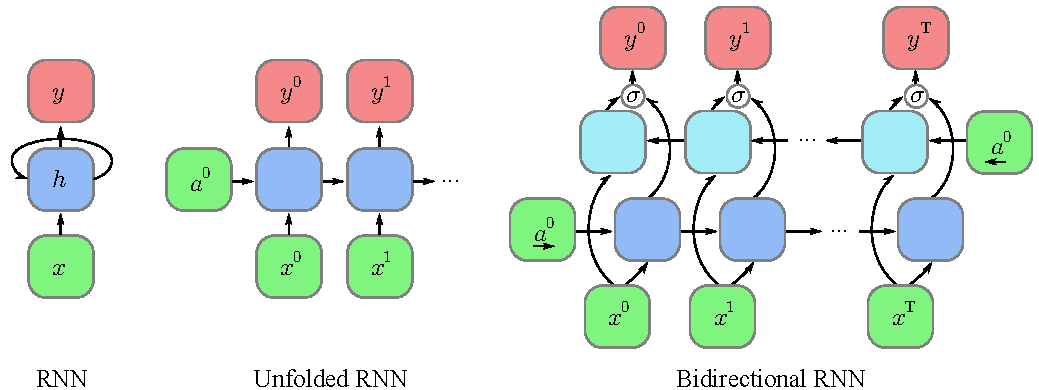
\includegraphics[width=\textwidth]{literature/imgs/2-RNN-unfold.pdf}
    \caption{RNN, unfolded unidirectional RNN and unfolded bidirectional RNN}
    \label{fig:2-RNN-unfold}
\end{figure}

%LSTM
However, \citet{hochreiter1997long} points out that simple RNN tends to only keep short-term memory and is prone to lose long-term memory, because the same weight of the network is shared at all time steps, and the final gradient tends to disappear after multiple time steps, proved by Hochreiter's analysis.

\begin{equation}
    \frac{\partial \vartheta_{v}(t-q)}{\partial \vartheta_{u}(t)}=\sum_{l_{1}=1}^{n} \ldots \sum_{l_{q-1}=1}^{n} \prod_{m=1}^{q} f_{l_{m}}^{\prime}\left(n e t_{l_{m}}(t-m)\right) w_{l_{m} l_{m-1}}
    \eqcite{hochreiter1997long}
    \label{equ:2-RNN-loss-scaled}
\end{equation}

Formula \ref{equ:2-RNN-loss-scaled} shows that the back-propagation gradient in simple RNN is equal to the product of the gradients of each time step after multi-step propagation.
An intuitive explanation is that the gradient is mainly dominated by the short-distance gradient, and thus it is difficult for the model to learn long-distance dependence.

Long-short-term memory (LSTM) is proposed to solve the problem that the simple RNN cannot learn long-term dependence by introducing a separated cell state $C_t$ to keep long-term memory. And later on, \citet{Gers2000LearningTF} introduce I/O gates, a forget gate to control loss or keep memory in cell state, resulted in the modern LSTM cell structure shown in the left of Figure \ref{fig:ext-LSTM-GRU}.

\begin{figure}[ht!]
    \centering
    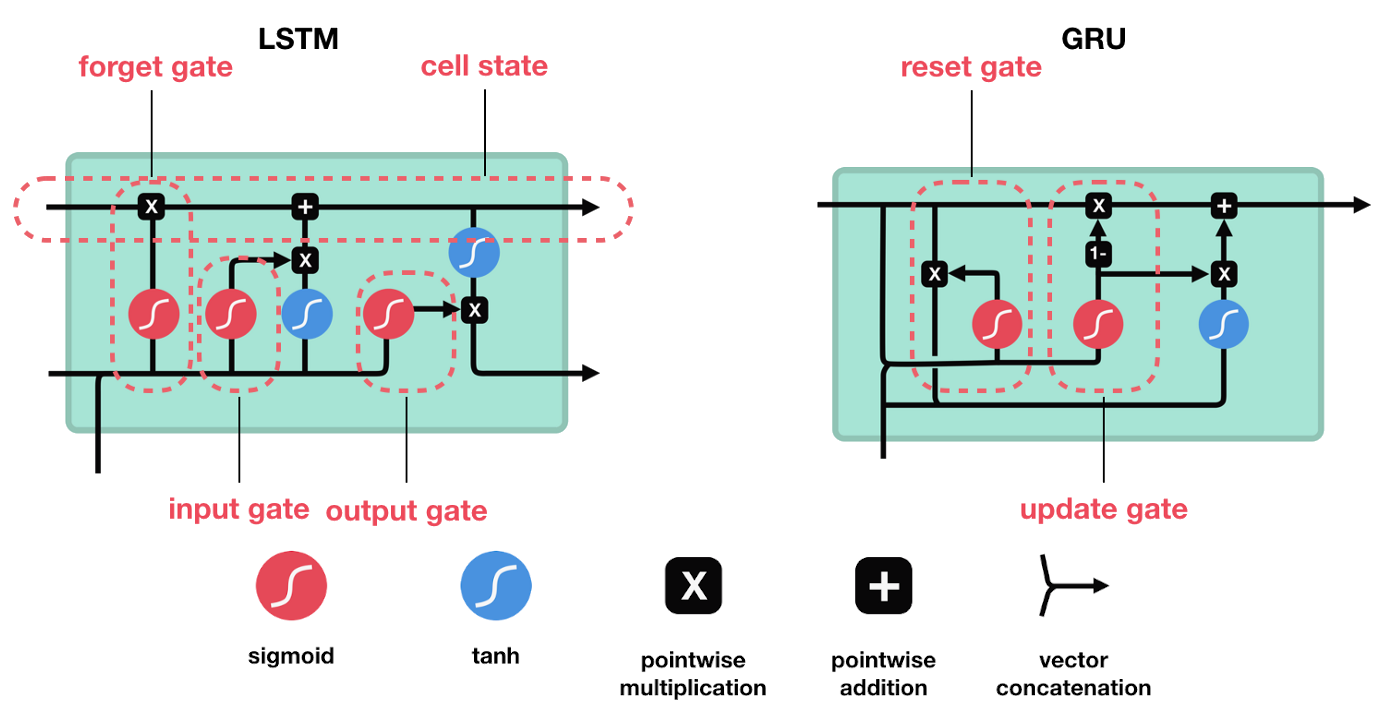
\includegraphics[width=.9\textwidth]{literature/imgs/ext-LSTM-GRU.png}
    \caption{LSTM and GRU structure comparison by \citet{phi2018illustrated}}
    \label{fig:ext-LSTM-GRU}
\end{figure}

%GRU
LSTM introduces lots of things into RNN, which leads to an increase in trainable parameters of each unit, making it harder to create a model with a deeper network.
Gated recurrent unit (GRU) is an improved LSTM algorithm proposed by \citet{chung2014empirical} in 2014. It merges the forget gate and the input gate into a single update gate. It also combines the cell state and the hidden state.
As shown in the right of Figure \ref{fig:ext-LSTM-GRU}, GRU structure is much simpler than LSTM, making it possible to create a deeper network.

LSTM and GRU only remedy and alleviate the problem of gradient vanish to a certain extent in RNN, and memory loss can still occur in the case of long-range dependencies.
Most importantly, this network structure has one limitation that made it not suitable for mobile applications.
The enforced sequential calculation process is due to dependencies on the result from the previous time, which greatly limits the parallel capability of calculations, thus making it impossible to achieve reasonable performance on mobile devices.
